% \documentclass{WHUBachelor}% 选项 forprint: 交付打印时添加, 避免彩色链接字迹打印偏淡. 即使用下一行:
 \documentclass[forprint]{WHUBachelor}
  \lstset{ 
    basicstyle=\small,% 
    escapeinside=``,% 
    keywordstyle=\color{red} \bfseries,% \underbar,% 
    identifierstyle={},% 
    commentstyle=\color{blue},% 
    stringstyle=\ttfamily,% 
    %labelstyle=\tiny,% 
    breaklines=true,
    extendedchars=false,% 
    linewidth=\textwidth,% 
    numbers=left,% 
    numberstyle=\tiny \color{blue},% 
    frame=trbl% 
    }


\begin{document}
%%%%%%% 下面的内容, 据实填空.

\title{实验项目三:具有独立内核的操作系统的实现}
\Cschoolname{数据科学与计算机学院}          % 学院名
\Cmajor{计算机科学与技术}                  % 专业中文名
\StudentNumber{16337237} % 填写自己的学号
\author{王永锋}                            % 作者名字
\Csupervisor{凌应标}        %指导教师中文名、职称
\date{二〇一八年三月三十一日}                % 日期, 要注意和英文日期一致!!

%----------------------------------------------------------------------------
\pdfbookmark[0]{封面}{title}         % 封面页加到 pdf 书签
\maketitle
\frontmatter
\pagenumbering{Roman}              % 正文之前的页码用大写罗马字母编号.
%-----------------------------------------------------------------------------
% \include{includefile/frontmatter}    % 加入摘要, 申明.
%==========================把目录加入到书签==============================%%%%%%
\pdfbookmark[0]{目录}{toc}
\tableofcontents
\mainmatter %% 以下是正文

%%%%%%%%%%%%%%%%%%%%%%%%%%%%%%%%%%%%%%%%%%%%%%%%%%%%%%%%%%%%%%%%%%%%%%%%%%%%%%%%%%%%%
%【实验方案】包括:硬件或虚拟机配置方法、软件工具与作用、方案的思想、相关原理、程序流程、算法和数据结构、程序关键模块,结合代码与程序中的位置位置进行解释。不得抄袭,否则按作弊处理。
%【实验过程】包括:主要工具安装使用过程及截图结果、程序过程中的操作步骤、测试数据、输入及输出说明、遇到的问题及解决情况、关键功能或操作的截图结果。不得抄袭,否则按作弊处理。
%【实验总结】每人必需写一段,文字不少于500字,可以写心得体会、问题讨论与思考、新的设想、感言总结或提出建议等等。不得抄袭,否则按作弊处理。
%【参考文献】(如有要列出,包括网上资源)
%%%%%%%%%%%%%%%%%%%%%%%%%%%--------main matter-------%%%%%%%%%%%%%%%%%%%%%%%%%%%%%%%%%%%%
\chapter{实验目的及要求}

\section{实验目的}

\begin{enumerate}
  \item 把原来在引导扇区中实现的监控程序(内核)分离成一个独立的执行体,存放在其它扇区中,为“后来“扩展内核提供发展空间。
  \item 学习汇编与c混合编程技术,改写实验二的监控程序,扩展其命令处理能力,增加实现实验要求2中的部分或全部功能。
\end{enumerate}

\section{实验要求}

本次实验,要求需要完成以下目标:\\

\begin{itemize}
  \item 规定时间内单独完成实验。
  \item 实验三必须在实验二基础上进行,保留或扩展原有功能,实现部分新增功能。
  \item 监控程序以独立的可执行程序实现,并由引导程序加载进内存适当位星,内核获得控制权后开始显示必要的操作提示信息,实现若干命令,方便使用者(测试者)操作。
  \item 制作包含引导程序,监控程序和若干可加载并执行的用户程序组成的1.44M软盘映像。
  \item 在指定时间内,提交所有相关源程序文件和软盘映像文件,操作使用说明和实验报告。
  \item 实验报告格式不变,实验方案丶实验过程或心得体会中主要描述个人工作,必须有展示技术性的过程细节截图和说明。
\end{itemize}

\chapter{实验方案}

\section{实验工具和环境}

本次实验平台\footnote{部分参考\cite{于渊2009orange}}搭建在win10系统的linux子系统上,通过编写makefile文件,连接nasm,gcc编译工具,dd二进制文件覆写工具,与bochs,qemu虚拟机加载配置文件与镜像(具体工具链详见下\autoref{tab:tools})。

与前几次实验相比,这一次实验代码的规模大了很多,仅仅凭借脚本并不容易将一整个项目进行高效的编译。因此,这一次我使用的是makefile来帮助这个项目进行自动化建构,只编译修改过的文件,而不编译不变的文件,以这种方式,加快了项目编译的速度,同时也能保证项目中各个文件之间的依赖关系不被破坏。

\begin{table}[htp]
  \caption{本实验所使用的工具链}
  \centering
  \begin{tabular}{cc}
    \toprule
    软件名称 & 用途  \\
    \midrule
    bash & 一个命令行终端,可提供linux的一些命令与执行shell脚本 \\
    nasm & 将x86汇编文件编译成.bin二进制文件 \\
    gcc & 编译工具,将c编译成二进制文件 \\
    ld & gcc套件中包含的连接器,用于将多个可执行文件连接起来 \\
    make & gcc套件中的工具,用于执行makefile文件 \\
    dd & 将二进制文件的内容写进软盘镜像中  \\
    objdump & 对可执行文件或二进制文件进行反编译 \\
    hexdump & 以十六进制形式查看软盘镜像文件 \\
    bochs & 虚拟机,用于加载装有自定义引导程序的软盘,使用软件模拟,速度不稳定  \\
    bochsdbg & 调试工具,用于给装有自定义引导程序的软盘文件进行调试 \\
    qemu & 虚拟机,用于加载装有自定义程序的软盘,使用硬件模拟,速度稳定且较快 \\
    \bottomrule
  \end{tabular}
  \label{tab:tools}
\end{table}

\section{相关基础原理}

\subsection{gcc与nasm的混合编程}

\subsubsection{32位与16位汇编代码的理解}

在gcc和nasm结合实现混编的过程中,其实遇到了不少的问题。但我认为,一个最大的问题在于对\textbf{32位汇编代码},\textbf{16位汇编代码}的区别的理解,与CPU在16位实模式下读取操作数,地址的方式的理解。

首先定义32位汇编代码,我认为的32位汇编代码,是\textbf{指使用了32位的寄存器,或者指令中的立即数是32位的,或操作32位的地址和操作数的指令}。而对16位汇编代码,也有类似的定义。

但是,在没有任何指令前缀的情况下,其实无论是32位的汇编代码还是16位的汇编代码,在机器指令级别上其实是看不出区别的。

这里说明一下,32位汇编指令和16位的汇编指令有以下共同点:

\begin{itemize}
  \item 操作码相同,如无论是从栈中取32位地址做返回地址的retl,还是从栈中取16位地址的ret,机器码都是0xc3。
  \item 寄存器索引相同。对于公有的寄存器,如ax,索引该寄存器的数字与索引eax寄存器的数字在机器指令层面是一致的。
\end{itemize} 

而32位汇编指令和16位汇编指令的差异在前面定义的时候已经讲得很清楚了,他们的差异主要体现在能在机器指令上看到的立即数的长度不同,还有隐含的处理器对寄存器或栈操作的行为的不同。


\begin{figure}[htp]
  \centering
  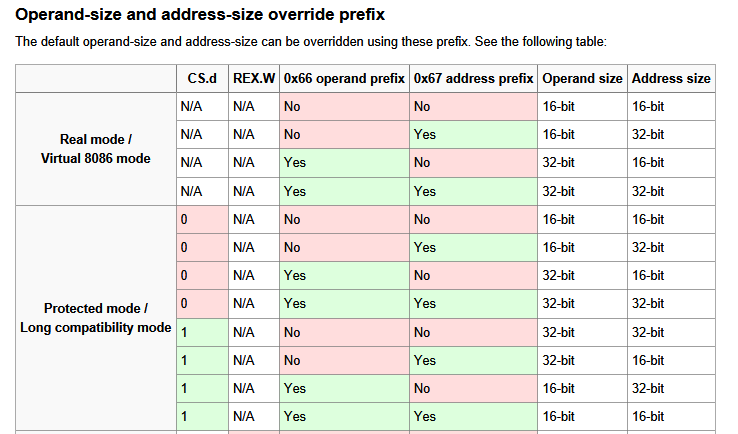
\includegraphics[width=11cm]{"./figure/wiki_prefix.png"}
  \caption{处理器在不同的模式下对指令的处理方式}
  \label{fig:wiki-prefix}
\end{figure}

当时想到这里,我就有一个特别特别严重的疑惑:从操作码上16位汇编指令和32位汇编指令完全相同,那么处理器自身是如何知道以何种方式(32/16)来处理这一些指令的呢?基于这样的疑惑,我在wiki上找到了这样的资料。TODO:引用


从这幅图中,可以看到,处理器处理指令的方式主要有两个因素来决定,一个是处理器当前所处模式,另一个是指令前缀的使用。\textbf{我们当前仍然处于16位实模式下,因此在没有任何前缀的情况下,处理器对指令的处理方式都是以16位的方式来进行处理的,而执行前若有0x66,0x67前缀,就意味着处理器在遇到这一条指令的时候,会使用32位的寄存器和操作数,或者处理指令中32位的地址。}

\subsubsection{实践中的验证}

之所以需要讲清楚32位汇编代码的共同点和差异点,是因为我们必须理解gcc生成的32位汇编代码与nasm产生的16位汇编代码之间的关系,同时认清CPU如何识别gcc生成的32位汇编代码,在理解的基础上,我们才能够有底气的使用这些工具给我们提供的各种功能,实现C与汇编交叉编译。

nasm 在使用bits 16 伪指令后,它能够生成16位的汇编指令,这些汇编指令有以下特点。

\begin{itemize}
  \item 操作码前没有前缀,处理器按16位实模式下默认方式工作。
  \item 指令长度较短,指令中的立即数长16比特,call指令中的偏移量长16比特。
  \item 在对栈进行操作的时候,push指令会把16位的操作数push进栈中。
  \item 操作的寄存器都是16位的。
\end{itemize}

gcc 在使用 -m16 选项编译后,他能够生成16位实模式下兼容的32位汇编指令,这些汇编指令有以下特点。

\begin{itemize}
  \item 操作码有前缀 0x66 或 0x67,表明处理器按照非默认方式(32位)读取操作数和地址。
  \item 指令长度较长,指令中的立即数长32比特,call指令中的偏移量长32比特。
  \item 对栈进行操作的时候,push指令会把32位的操作数push进栈中。
  \item 操作32位的寄存器(如eax等)
\end{itemize}

这些指令在机器代码上的区别可见图\autoref{fig:nasm-16asm},\autoref{fig:gcc-32asm}。

\begin{figure}[htp]
  \centering
  \begin{minipage}[t]{0.5\linewidth} 
  \centering
  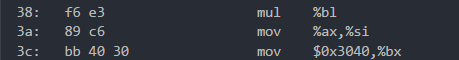
\includegraphics[width=10cm]{"./figure/nasm_16asm.png"}
  \caption{nasm生成的16位汇编代码}
  \label{fig:nasm-16asm}
  \end{minipage}

  \begin{minipage}[t]{0.5\linewidth} 
  \centering
  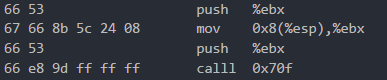
\includegraphics[width=10cm]{"./figure/gcc_32asm.png"}
  \caption{gcc生成的32位汇编代码}
  \label{fig:gcc-32asm}
  \end{minipage}
\end{figure}

在这里,我们证实了以下两个结论:

\begin{itemize}
  \item 无论是gcc,还是nasm,只要使用恰当的编译指令产生的机器指令,都能够在16位实模式下正确运行。
  \item nasm与gcc产生的汇编代码,在相互调用的时候可能会产生问题,问题主要在c的call是push32位地址,而nasm的ret是取16位地址。一来一回就会产生问题。
\end{itemize}

\subsubsection{gcc和nasm产生可执行文件的可连接性}

上面证实了指令的可运行性,这里在确认一下两种可执行文件的可连接性。

要保证两种可执行文件可以连接,必须保证两种文件有着相同的可执行文件的格式。所幸,通过搜寻资料,我发现nasm在使用-f elf32的情况下能够输出elf32格式的可执行文件,gcc在-m16的默认情况下输出一种格式为elf32的可执行文件,同时,连接器也支持使用-m elf\_i386的指令,连接两个elf32格式的可执行文件,这就为最终连接成功奠定了基石。

同时,考虑到最终生成的可执行文件还不能直接写入软盘,我们还需要生成不包含文件头的纯二进制文件,对于这个需求,ld工具中控制输出格式的一个参数--oformat binary可以用来控制输出文件的格式。

以下是编译指令样例

\begin{lstlisting}
  nasm -f elf32 -o kernel.o kernel.asm
  gcc -c -m16 -ffreestanding -o start.o start.asm
  ld -Ttext 0x00000 -m elf_i386 --oformat binary -o kernel.bin kernel.o start.o
\end{lstlisting}

在上面有两个指令没有说明的,一个是gcc中的-ffreestanding ,这个指令的用途是表明这个程序没有用到任何库函数,不能够对库函数做优化;另一个是 ld工具的-Ttext 0x00000 ,他的作用与org类似。

同时,还有一个显而易见不需要说明的是,代码中必须有global,extern等关键词用作将名字导出或导入,这样之后的连接器才能够正确识别并连接。不过,由于elf格式的特殊性,名字在编译后不会产生下划线前缀(TODO:NASM文档)

至此,C与汇编混合编程完成。

\subsubsection{gcc和nasm下c与汇编混合编程的方法}

在证实指令的运行性和可连接性后,对两个不同的编译器产生的有一点点相互不兼容的地方,我们做以下妥协,保证代码的正确运行。

\begin{itemize}
  \item 为确保统一,代码中出现的call和ret统一显式指明使用32位格式。具体的方式是:
  \begin{lstlisting}[language={[x86masm]Assembler}]
    ; 使用宏,在ret指令前显式添加0x66前缀
    %macro retl 0
    db 0x66
    ret
    %endmacro
    ; 在call的时候添加 dword,确保call产生32位的偏移量。
    call dword LABEL
  \end{lstlisting}

  \item gcc生成汇编代码的过程中,可能会生成用到段寄存器的指令(如从数据段获取数据)。这里我们需要了解gcc一般会默认cs,ss,ds,es等段寄存器都是一致的。因此在跳入C代码段的时候,要确保段寄存器的一致性。

  \item gcc遵循C调用约定(TODO:WIKI),因此关于参数传递以及返回值的规范需要汇编代码遵守。
  
\end{itemize}

\section{程序功能说明及大致思路阐述}

这里会对程序的大致运行流程进行一个粗略的描述,同时罗列了当前系统内核支持的功能。

\subsection{程序大致思路阐述}

\begin{enumerate}
  \item 一开机,处于软盘第一个扇区的引导程序加载第72-89个扇区,作为系统内核,并将控制权转交给系统内核。
  \item 系统内核刚开始运行,经过一系列初始化工作(如安装中断,加载fat表,根目录表),跳转到tty例程(即用户终端。
  \item 进入到命令行中断,系统管理员可以在这里执行一系列指令 TODO:
\end{enumerate}

\subsection{程序功能说明}
TODO:对程序功能需要进一步完善。
本程序(完整程序代码见附件)实现了以下功能(主界面可见\autoref{fig:main_screen})。
\begin{enumerate}
  \item \textbf{按下1。}
\end{enumerate}

\section{代码框架及依赖}

TODO:想画一幅图,展现代码文件之间的依赖。

TODO:好好想一下怎么说明代码的组织方式。

\chapter{实验结果}

\section{系统内核主菜单}

TODO:功能的展示。
本程序经nasm,gcc编译后在qemu虚拟机下运行的效果可见\autoref{fig:main_screen}与\autoref{fig:main_screen2},其中\autoref{fig:main_screen2}中的边框可以逆时钟旋转同时随机地改变颜色。
\begin{figure}[htp]
  \centering
  \begin{minipage}[t]{0.5\linewidth} 
  \centering
  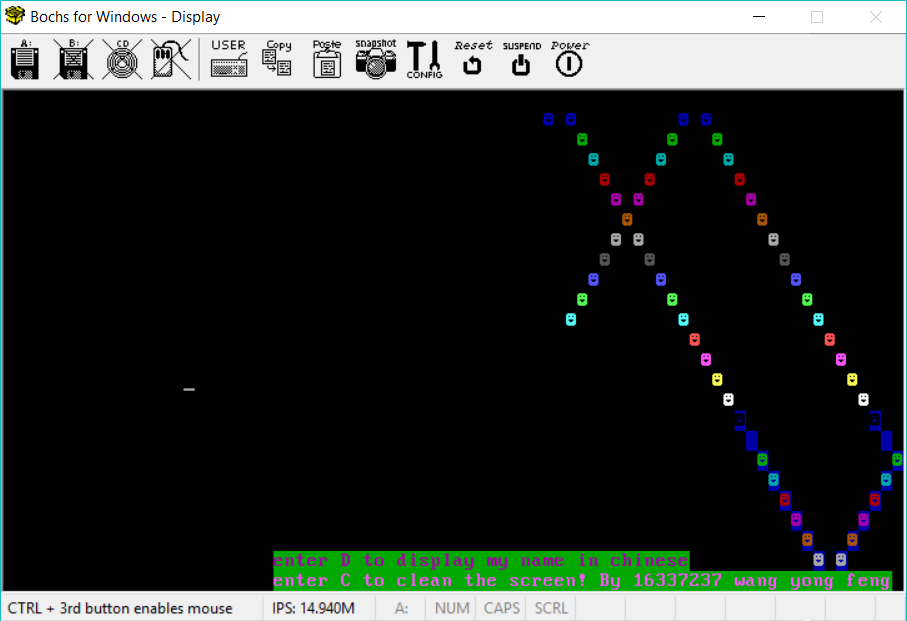
\includegraphics[width=10cm]{"./figure/main_screen.png"}
  \caption{命令行终端的主界面}
  \label{fig:main_screen}
  \end{minipage}

  \begin{minipage}[t]{0.5\linewidth} 
  \centering
  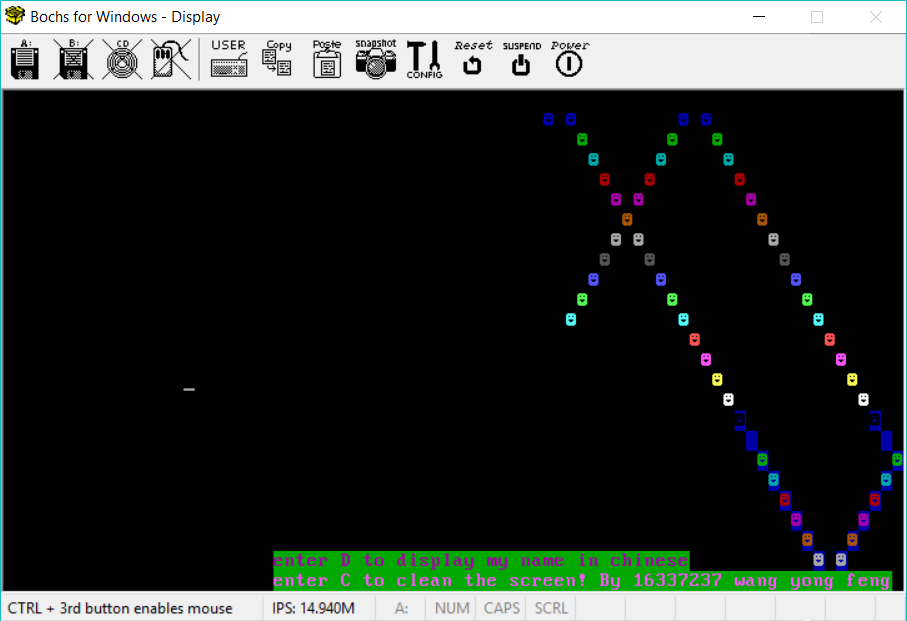
\includegraphics[width=10cm]{"./figure/main_screen.png"}
  \caption{自定义引导程序按下D后的界面}
  \label{fig:main_screen2}
  \end{minipage}
\end{figure}


\chapter{实验总结}

这是实验三的实验总结。

在实验前期,我对c与汇编混合编程的概念并不了解。在一开始接触到混合编程的时候,甚至是想了半天为什么要使用c语言和汇编混合编程,还想了很久需要使用C语言做什么事情,紧接着,对C语言中隐藏的细节再进行了很多的思考,以想明白如何使用c语言替换汇编的代码。

C语言,可以说是已经很贴近硬件底层的语言了,可是直到我将C语言与汇编语言结合起来使用,我才更进一步的认识到C语言对内存的操控,

%%%============================================================================================================%%%

%%%=== 参考文献 ========%%%



% \cleardoublepage\phantomsection
% \addcontentsline{toc}{chapter}{参考文献}

\bibliography{opsystem}
% \bibliographystyle{unsrt}

% \begin{thebibliography}{00}

%   \bibitem{r1} 作者. 文章题目 [J].  期刊名, 出版年份,卷号(期数): 起止页码.

%   \bibitem{r2} 作者. 书名 [M]. 版次. 出版地:出版单位,出版年份:起止页码.

%   \bibitem{r3} 邓建松等, 《\LaTeXe~科技排版指南》, 科学出版社.

%   \bibitem{r4} 吴凌云, 《CTeX~FAQ (常见问题集)》, \textit{Version~0.4}, June 21, 2004.

%   \bibitem{r5} Herbert Vo\ss, Mathmode, \url{http://www.tex.ac.uk/ctan/info/math/voss/mathmode/Mathmode.pdf}.


% \end{thebibliography}

% \include{includefile/backmatter} %%%致谢

%%%-------------- 附录. 不需要可以删除.-----------
\appendix

\chapter{运行汇编文件的脚本}
\label{code:my_shell}
这是我为了方便,在win10平台下的bash终端编写的shell脚本。前面编译环节,能够保证一旦发生编译错误,就停止运行,不打开虚拟机。
\begin{lstlisting}
  nasm.exe -f bin my_mbr.asm -l my_mbr.list -o my_mbr.bin    || { echo "nasm complied failed"; exit 1; }
  nasm.exe -f bin my_core.asm -l my_core.list -o my_core.bin   || { echo "nasm complied failed"; exit 1; }
  nasm.exe -f bin my_user_program_1.asm -l my_user_program_1.list -o my_user_program_1.bin   || { echo "nasm complied failed"; exit 1; }
  nasm.exe -f bin my_user_program_2.asm -l my_user_program_2.list -o my_user_program_2.bin   || { echo "nasm complied failed"; exit 1; }
  nasm.exe -f bin my_user_program_3.asm -l my_user_program_3.list -o my_user_program_3.bin   || { echo "nasm complied failed"; exit 1; }
  nasm.exe -f bin my_user_program_4.asm -l my_user_program_4.list -o my_user_program_4.bin   || { echo "nasm complied failed"; exit 1; }
  nasm.exe -f bin my_user_program_l.asm -l my_user_program_l.list -o my_user_program_l.bin   || { echo "nasm complied failed"; exit 1; }
  nasm.exe -f bin my_user_program_t.asm -l my_user_program_t.list -o my_user_program_t.bin   || { echo "nasm complied failed"; exit 1; }
  dd if=/dev/zero of=a.img ibs=512 count=100 conv=notrunc
  dd if=my_mbr.bin of=a.img ibs=512 count=1 conv=notrunc
  dd if=my_core.bin of=a.img ibs=512 count=10 conv=notrunc seek=1
  dd if=my_user_program_1.bin of=a.img ibs=512 count=10 conv=notrunc seek=18
  dd if=my_user_program_2.bin of=a.img ibs=512 count=10 conv=notrunc seek=36
  dd if=my_user_program_3.bin of=a.img ibs=512 count=10 conv=notrunc seek=54
  dd if=my_user_program_4.bin of=a.img ibs=512 count=10 conv=notrunc seek=72
  dd if=my_user_program_l.bin of=a.img ibs=512 count=10 conv=notrunc seek=90
  dd if=my_user_program_t.bin of=a.img ibs=512 count=10 conv=notrunc seek=108
  
  case $1 in
  b)
  bochs.exe -q
  ;;  
  q)
  qemu-system-i386.exe -fda a.img
  ;;  
  d)
  bochsdbg.exe -q  
  ;;  
  *)
  echo "Usage: $name [b|q|d]"  
  exit 1  
  ;;  
  esac
  
  rm *.bin
  rm *.list
  rm bochsout.txt
\end{lstlisting}

\chapter{内核代码段入口}

\label{code:my_core_entry}
\begin{lstlisting}[language={[x86masm]Assembler}] 
  code_start:
  ; 先进行清屏
call clean_screen
  ; 初始化内核段地址
  ; 此时ds指向header
  ; cs 指向正确的位置。
  mov ax, ds
  mov es, ax
  ; es 指向header
  mov ax, [stack_segment]
  mov ss, ax
  mov sp, stack_end
  mov ax, [data_segment]
  mov ds, ax

  ; 安装中断
  ; 安装40号中断,用于返回
  call install_int40
  call install_int8
  ; 内核已加载完成,按enter继续
  call display_core_massage



check_key_board_load_core:
  mov ah, 01h
  int 16h
  ; 不断查询键盘缓冲区的状况
  ; 若有按键,则zf为0,若无按键,则zf为1,跳回去继续查询
  jz check_key_board_load_core
  ; 有字符输入
  mov ah, 00h
  int 16h

  cmp al, 0x0d
  jnz check_key_board_load_core
  
check_key_board_load_core_end:


;----------------------------内核功能入口---------
core_start:
  call clean_screen
  call show_welcome_screen
; 这里放的是内核加载器,负责加载在其他扇区的程序。
check_key_board_load_feature:
  mov ah, 01h
  int 16h
  ; 不断查询键盘缓冲区的状况
  ; 若有按键,则zf为0,若无按键,则zf为1,跳回去继续查询
  jz check_key_board_load_feature
  ; 有字符输入,从al中读取键盘输入
  mov ah, 00h
  int 16h

check_key_board_load_feature_1:
  cmp al, '1' 
  jnz check_key_board_load_feature_2
  mov ax, 18 
  jmp run_com
check_key_board_load_feature_2:
  cmp al, '2' 
  jnz check_key_board_load_feature_3
  mov ax, 36
  jmp run_com
check_key_board_load_feature_3:
  cmp al, '3' 
  jnz check_key_board_load_feature_4
  mov ax, 54
  jmp run_com
check_key_board_load_feature_4:
  cmp al, '4' 
  jnz check_key_board_load_feature_l
  mov ax, 72
  jmp run_com
check_key_board_load_feature_l:
  cmp al, 'l' 
  jnz check_key_board_load_feature_t
  mov ax, 90
  jmp run_com
check_key_board_load_feature_t:
  cmp al, 't' 
  jnz check_key_board_load_feature
  mov ax, 108
  jmp run_com
  jmp check_key_board_load_feature

; 根据al里面的值加载对应的用户程序
run_com:
  call load_com_user_program
  jmp run_com_user_program

;###############################################
;------------------------------常用过程---------
; 运行用户com程序前运行
; 效果:
; 将cs,ds,es,ss置为0x1000
; 将sp置为0x0400(相当于.com程序末尾)
run_com_user_program:
  call clean_screen
  mov ax, 0x1000
  mov ds, ax
  mov es, ax
  mov ss, ax
  mov ax, 0x0400
  mov sp, ax
  jmp 0x1000:0x0000
;-------------------------------------------
\end{lstlisting}




\chapter{中断int 40h 的安装与执行}

\label{code:int40h}
\begin{lstlisting}[language={[x86masm]Assembler}]
  ; 安装40号中断,用于用户程序返回内核
  install_int40:
      push ax
      push bx
      push ds
  
      ; 安装 int 40 主要代码
      mov ax, 0
      mov ds, ax
      mov ax, cs
      mov word [0x40*4], int40_for_return 
      mov word [0x40*4+2], ax
      
      pop ds
      pop bx
      pop ax
      ret
  
  ; 40号中断的功能是将控制权从用户程序转到内核
  ; 务必要设计好0x40号中断,设计成与CPU状态无关,不依赖段寄存器的值
  ; 因为无论段寄存器是何值,都有可能会运行这条程序
  ; 执行中断的时候会将地址还有符号寄存器存到堆栈中
  ; 考虑先将堆栈中的东西pop出来,然后转移堆栈到内核栈,
  ; 修改各段指针后,再push内核的cs和指令偏移地址,通过iret回到内核
  int40_for_return:
  
      ; 在用户栈中
      pop ax ; pop 原调用中断的偏移地址
      pop ax ; pop 原调用中断的段地址
      pop bx ; pop 用户的标志寄存器
  
      ; 修改段寄存器:ds, ss, es
      mov ax, core_header_data_segment
      mov ds, ax
      mov es, ax
      mov ax, word [core_stack_segment_header_offset]
      mov ss, ax
      mov sp, core_stack_length
  
      ; 保证栈为内核状态
      push bx ; push 标志寄存器 可能要修改
      push word [core_code_segment_header_offset]
      push word [core_entry_header_offset]
  
      ; 设置数据段寄存器
      mov ax, [core_data_segment_header_offset]
      mov ds, ax
  
      ; 可以运行任何在内核态的程序啦
      call clean_screen
  
      iret ; 成功回到内核
  
\end{lstlisting}

\chapter{笑脸弹跳的代码}

\label{code:jump}
\begin{lstlisting}[language={[x86masm]Assembler}]
  loop1:
	dec word[count]			; 递减计数变量
	jnz loop1					; >0:跳转;
	mov word[count],delay
	dec word[dcount]			; 递减计数变量
      jnz loop1
	mov word[count],delay
	mov word[dcount],ddelay

check_keyboard:
    mov ah, 01h
    int 16h
    ; 不断查询键盘缓冲区的状况
    ; 若有按键,则zf为0,若无按键,则zf为1,跳回去继续查询
    jz clean_current_char
    ; 有字符输入,从al中读取键盘输入
    mov ah, 00h
    int 16h

    cmp al, 'q' ; 如果键入q则退出
    jnz check_keyboard
	int 40h
clean_current_char: ; 清除当前字母所占显存位置,准备画下一个字母显存
      xor ax,ax                 ; 计算显存地址
      mov ax,word[x]
	mov bx,80
	mul bx
	add ax,word[y]
	mov bx,2
	mul bx
	mov bx,ax
	mov ah,07h				
	mov al,20h		
	mov [gs:bx],ax  		;  显示字符的ASCII码值

check_x:
    mov ax, user1_bound_x_up
    cmp word [x], ax
    jz toggle_x_direct
    mov ax, user1_bound_x_down
    cmp word [x], ax
    jz toggle_x_direct
    jmp check_y
toggle_x_direct:
    mov ax, 0
    sub ax, word [x_direct]
    mov word [x_direct], ax
check_y:
    mov ax, user1_bound_y_left
    cmp word [y], ax
    jz toggle_y_direct
    mov ax, user1_bound_y_right
    cmp word [y], ax
    jz toggle_y_direct
    jmp char_move
toggle_y_direct:    
    mov ax, 0
    sub ax, word [y_direct]
    mov word [y_direct], ax

char_move:
    mov ax, word [x_direct]
    add word [x], ax
    mov ax, word [y_direct]
    add word [y], ax
show:	
    xor ax,ax                 ; 计算显存地址
    mov ax,word[x]
	mov bx,80
	mul bx
	add ax,word[y]
	mov bx,2
	mul bx
	mov bx,ax
	mov ah,bh				;  0000:黑底、1111:亮白字(默认值为07h)
	mov al,byte[char]			;  AL = 显示字符值(默认值为20h=空格符)
	mov [gs:bx],ax  		;  显示字符的ASCII码值
	jmp loop1
\end{lstlisting}


\cleardoublepage
\end{document}